\documentclass{article}
\usepackage{pgfplots}
\begin{document}
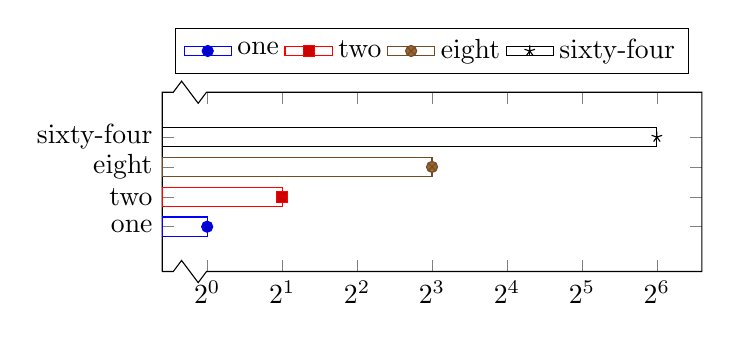
\begin{tikzpicture}
%\tracingmacros=2 \tracingcommands=2
\begin{semilogxaxis}[
 axis x discontinuity=crunch,
 log basis x=2,
 log origin=infty,
 y post scale=0.4,
 legend style={at={(0.5,1.1)},anchor=south},
 legend columns=4,
 ytick={one,two,eight,sixty-four},
 symbolic y coords={one,two,eight,sixty-four},
 bar width=7pt,
 enlarge y limits=0.5 
]

\addplot+[xbar] coordinates {(1,one)};
\addlegendentry{one}

\addplot+[xbar] coordinates {(2,two)};
\addlegendentry{two}

\addplot+[xbar] coordinates {(8,eight)};
\addlegendentry{eight}

\addplot+[xbar] coordinates {(64,sixty-four)};
\addlegendentry{sixty-four}

\end{semilogxaxis}
\end{tikzpicture}
\end{document}
